%*******************************************************
% Findings
%*******************************************************

\chapter{Results}
\par The findings from our fieldwork and data analysis are presented in this chapter. It is our hope that they will help improve and promote the installation of renewable thermal heating and cooling systems. We first discuss the metrics used when collecting data, then present the most relevant aspects of each of the following DOER-sponsored renewable thermal project sites we investigated: the Amherst College bunker building, the Southern Berkshire Regional School, and the Sudbury Public Housing Development. We then provide the list of findings we compiled from our data collection at each of the three project sites.

\section{Determination of Metrics}
\par Before visiting each project site to collect data, we needed to determine which metrics we would use in our analysis of the project. To determine these metrics, we met with our sponsor and point of contact at the DOER. We spoke with her about what concerns and questions the DOER has encountered working with past renewable thermal heating and cooling project sites. From this interview, we identified the following findings.

\subsection{Cost is a Metric for Assessing Renewable Thermal Projects}
\par In our interview with our sponsor, we asked what she thought were the main concerns of potential project site leaders when considering implementing a renewable thermal project. Her response was “A lot of it is cost, I think. They [potential project site leaders] want to know how much it is going to cost.” She then elaborated that project sites “request funding for the amount presented on the feasibility study. Say it’s underestimated and the bids come in at \$100,000 more; the project sites are in a bind because they only asked for funding up to what the feasibility study presented.”

\subsection{Community Acceptance is a Metric for Assessing Renewable Thermal Projects}
\par Community acceptance was also presented to us by our sponsor as an important metric to be considered and investigated when talking to project sites. Our sponsor states “Community acceptance is also important because they have to go to town meetings or the school board in order to get approval for something like this so they have to sell it.”

\subsection{Operational Logistics and Aesthetics are Metrics for Assessing Renewable Thermal Projects}
\par Operational logistics (pellet delivery for biomass systems) and aesthetics were also brought to our attention from our interview with our sponsor. She states “Space and aesthetics regarding the silo are also concerns that I have seen. Where the silo would go, how they would get the delivery, price of the pellets, and pellet availability.”

\section{Site Descriptions}
\par After determining which metrics we would be focusing on, we began gathering data for each project site. For each project site, we compiled a document containing information we would need to collect relating to each metric and the decision making process, and included information we already had access to in the feasibility studies from each site. We took this information gathering guide, found in Appendix 4, to each site in order to ensure that we collected all the information necessary to compile case studies.

\subsection{Amherst College Bunker Building}
\par Amherst College is a privately funded university that has an off campus book storage bunker. This bunker is 50,000 ft\textsuperscript{2} and must be climate controlled 24 hours a day, 7 days a week, for the entire year. The bunker is climate controlled year round in order to ensure that the integrity of the books, especially the antique books, is not compromised. In order to supply a proper climate for these books, the building is first cooled to remove moisture from the air and is then heated to achieve room temperature. Prior to the installation of the new biomass boilers, this bunker was cooled with a stand alone air conditioning system and heated with two 15 year old Burnham cast iron, oil boilers, each rated at 560,000 BTU/hour. The facility’s management has greatly reduced its energy use in recent years by increasing the range of temperatures and humidity allowed within the building and decreasing ventilation. We interviewed an individual who worked closely with the project process and continues to work with the maintenance of the system in order to gather the information presented in the following sections.
\begin{figure}[H]
\centering
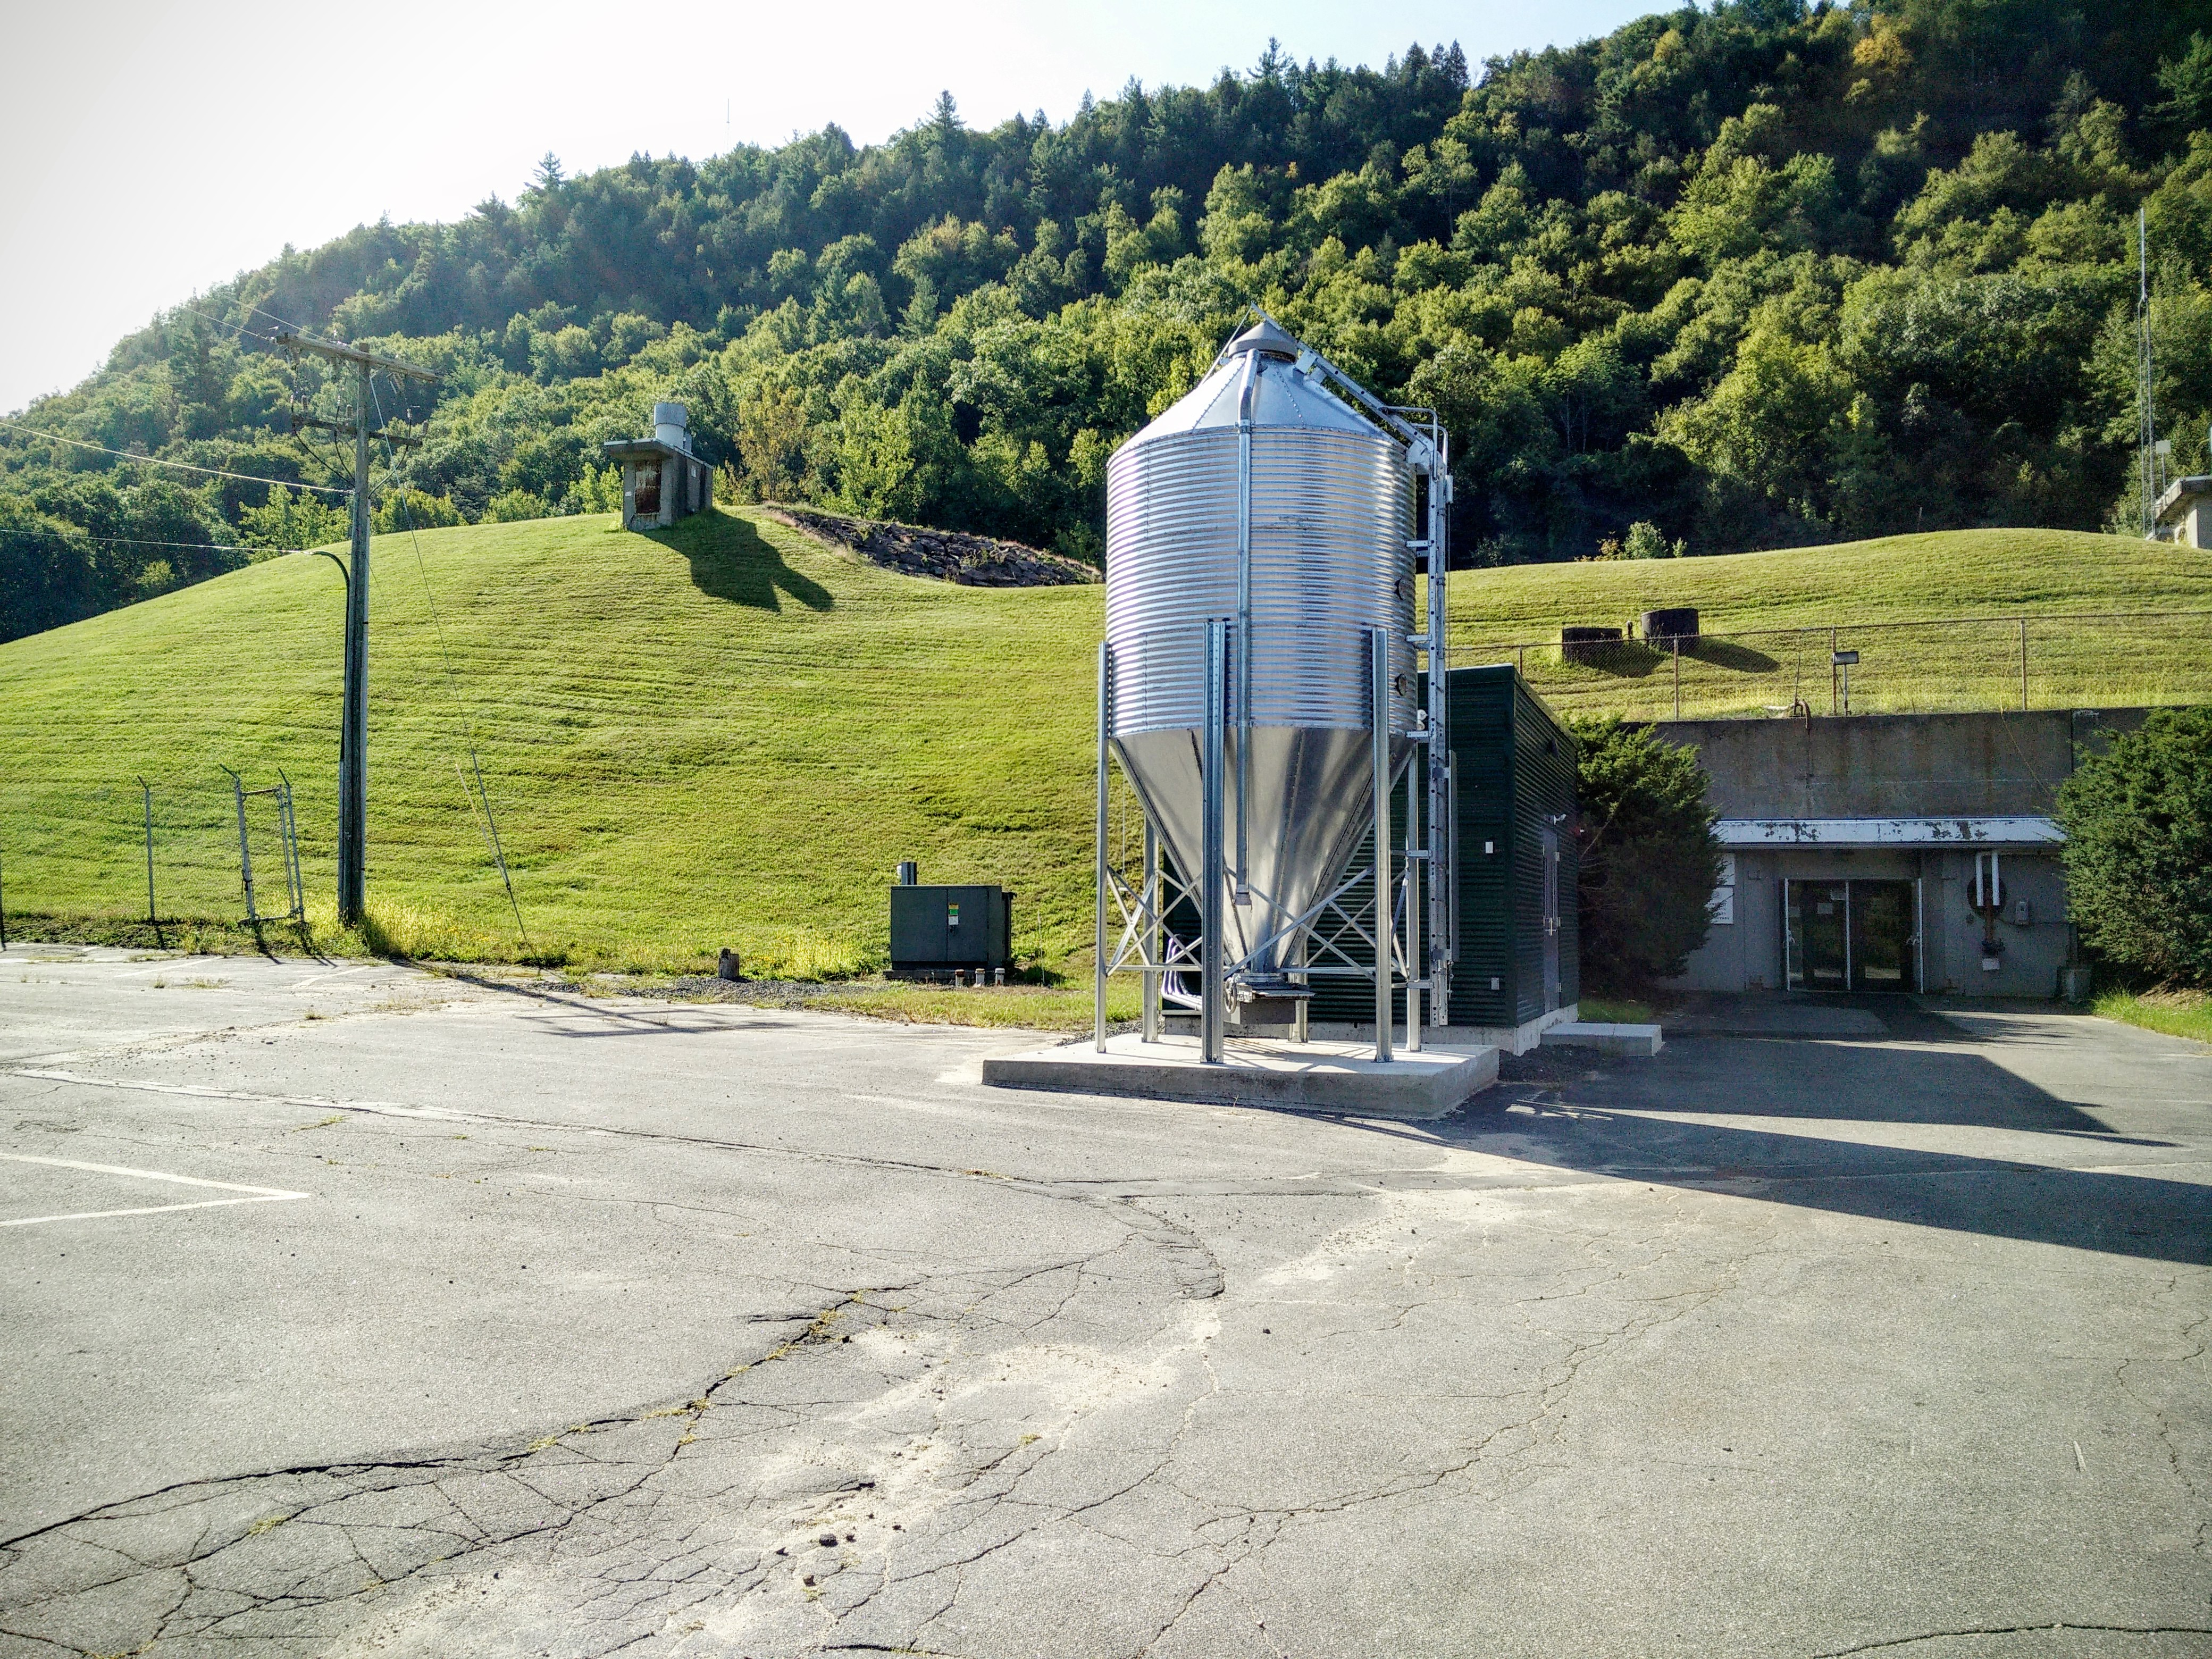
\includegraphics[width=0.75\textwidth]{findingschapter/amherstbuilding}
\caption{Amherst College Bunker Building}
\end{figure}

\subsubsection{The Introduction of Renewable Technology to Amherst College}
\par Amherst College applied for a grant through the DOER when their oil boilers were approaching end of life expectancy. When considering their options for heating this space, they contacted an outside contractor to become informed about the different heating options available on the market. Initially, the project site leader considered the implementation of a propane heating system. Upon discussing with this outside contractor, the idea of a biomass system was suggested due to the availability of a grant through the DOER. They applied for this grant with the help of the consulting firm, and once it was received, the decision was made. They were granted 75\% of the expected cost of the biomass boiler project, equating to \$205,000 out of the expected \$275,000.
\par After the engineers analyzed the load of the building and the usage patterns, they determined that two biomass boilers would be ideal. Having two boilers provides a 100\% redundancy which allows them to shut off one boiler for maintenance while the other still fully heats the building. After considering the space available inside the old oil boiler building, the consulting firm determined that building a new boiler room closer to the bunker would be the best option. A closer boiler room would decrease the amount of piping required and allow the old oil boilers to be operational during construction. This new boiler building would also allow for a 600 gallon thermal storage tank sized to fit the load of the building.
\begin{figure}[H]
\centering
\includegraphics[width=0.75\textwidth]{findingschapter/amherstboilerroom}
\caption{Amherst College New Boiler Building}
\end{figure}

\subsubsection{Aesthetics and Operational Logistics}
\par The biomass boilers require nearby pellet storage to allow for easy access to the fuel source. Amherst College chose to use a silo for their on-site storage rather than construct an indoor pellet storage bin. When implementing a biomass heating and cooling system, silo aesthetics often come up as a point of contention. Silos are rather large and can obstruct from the aesthetic quality of the building. Since the bunker building at Amherst College is off campus and in a remote location, aesthetics were not of concern. The silo at Amherst is 12’ in diameter by 26’ tall. The sizing of the silo provides enough room for 4 to 5 months worth of pellet storage which allows them to buy pellets in bulk and save money on delivery charges as they only have to get delivers 2-3 times a year. Depending on the site, delivery logistics can be a concern. A requirement for a biomass system is that the space/roadways allow for a large truck to provide wood pellet deliveries to the silo. The bunker building has ample parking space surrounding the silo and bunker building, so there were no issues with delivery logistics.
\begin{figure}[H]
\centering
\includegraphics[width=0.75\textwidth, angle=-90]{findingschapter/amherstsilo}
\caption{Silo at Amherst College}
\end{figure}

\subsubsection{Construction}
\par Amherst College was referred to Froling Energy for the construction by the same contractor who referred them to DOER for the grant. Although the construction was set to begin on October 2nd, 2014, due to delays in the design process and in getting permits from the town, it was not actually started until December. The chosen boilers were produced by Froling, an Austrian company with no relation to the energy company based in New Hampshire. Froling has been described as “the Cadillac of biomass boilers” by the DOER’s resident biomass expert. Construction was set to be completed by November \nth{26} 2014, but the boilers were not fully online until April \nth{1}, 2015. The process of installation required digging trenches in order to lay down piping from the new boilers to the bunker building. The timeline delay was a result of the harsh winter experienced in 2014 which inhibited the ability of the contractors to dig the necessary trenches.

\subsubsection{Current Operations and Maintenance}
\par The boilers have been operational for approximately six months as of September, 2015. As part of the maintenance requirements for biomass boilers, an ashtray is to be emptied every 6-8 weeks. Besides that, it is very similar to the oil boilers with an annual cleaning, annual inspections and weekly checkups. Additionally, the old oil boiler system produced a coating of soot that had to be removed each year whereas the biomass boilers produce only a thin layer of biodegradable wood dust from the pellets that can be easily removed. To aid in the maintenance process, the boilers are equipped with sensors that monitor different components of the system. Amherst College has a contract with Froling Energy to remotely supervise the system through these sensors and notify the facilities faculty if any abnormality occurs. In general, the new biomass system has a comparable maintenance schedule to the old oil boilers, and with time and experience, the Amherst facilities personnel expect it to become a faster and cleaner process.
\begin{figure}[H]
\centering
\includegraphics[width=0.75\textwidth]{findingschapter/amherstboilers}
\caption{Froling Boilers at the Amherst College Bunker Building}
\end{figure}

\subsubsection{Lessons Learned}
\par From our interview and onsite visit at the Amherst College Bunker Building, we developed a list of “lessons learned” that will be included in our case studies. The first lesson learned from this project site is to seek an experienced team. Amherst College was fortunate to work with experienced engineers throughout this project which allowed for a relatively smooth project process. Wood pellet boilers are relatively new to the United States, though the industry is well developed in Europe. Because of key differences in operation between wood pellet and fossil fuel systems-such as longer startup and shutdown times and the importance of thermal storage- working with engineering firms with relevant experience makes a renewable thermal project process run more smoothly.
\par The second lesson learned from the Amherst College Bunker Building is that the timeline for these projects can change even when working with experienced engineers. Construction was set to take place between October 2nd-November26th. Due to delays in the design process, construction began in December. As the construction occurred in the winter, there were weather related setbacks and the biomass system was not placed online until April 1st. However, due to proper planning and preparation, this delay did not affect the bunker’s ability to maintain proper climate for the books. Since the project involved constructing a separate boiler building, the school was able to use their old oil boilers throughout the project installation process.

\subsubsection{Site Summary}
\par Overall, the Amherst College biomass installation was a successful project. The staff and project coordinators are very happy with the project process and the performance of the new boilers. The individual we interviewed from Amherst College expressed that they are very pleased with the contractors they used to install the boilers, and the boilers themselves. The individual states“In the short time that we’ve had this system up and running, we are pretty impressed with it. I think we’re glad that we made the decision to go with this and we are looking forward to many years of trouble free operation years of trouble free operation.” He mentioned that they were comforted knowing that Froling Energy was familiar with the technology and the installation process. The advanced sensor system of the Froling boilers allows for remote access to information regarding maintenance needs, and the maintenance of the system is comparable to that of their old system. Cost was a concern for the stakeholders at Amherst College, but with funding from the DOER, the project became very affordable. The timeline for the project did shift, and the installation did take longer than expected, but since this construction involved creation of a new building for the biomass boilers, the old oil boilers were able to maintain the climate of the bunker building throughout the construction process. Aesthetics were not a concern for this project due to the off-campus location of the bunker building.

\subsection{Southern Berkshire Regional School}
\par The Southern Berkshire Regional School is a public school in Sheffield, Massachusetts. It is a 220,000 ft.\textsuperscript{2} building that is comprised of a high school and an elementary school separated in two wings. The building serves a total of 845 students, faculty, and staff. Originally the school was equipped with two oil boilers, providing 9.146 billion BTUs of heating annually, which were approaching the end of their lifespan and would need to be replaced. The school district looked towards a grant provided by the Massachusetts School Building Authority through their Accelerated Repairs Program to help fund new boilers and a new roof, another renovation that needed to be done at the time. During this grant search, they found the DOER SAPHIRE program, which introduced them to the idea of using a renewable energy production method such as biomass or geothermal heating. We interviewed two individuals who worked very closely with acquiring the grants from the DOER as well as communicating with the contractors prior to project implementation to obtain the information presented in the following sections.
\begin{figure}[H]
\centering
\includegraphics[width=0.75\textwidth]{findingschapter/southernberkshireschool}
\caption{Aerial View of the Southern Berkshire Regional School}
\end{figure}

\subsubsection{The Introduction of Renewable Technology to Southern Berkshire Regional School}
\par After school project leaders spoke with the DOER about the different potential renewable technology options, they decided to commission a feasibility study. This study, completed by BEAM engineering, compared the installation of a biomass system to the installation of a geothermal heat pump system. This study quickly found that a geothermal heat pump system would have been prohibitively expensive, as it normally is in retrofit scenarios.  Therefore, they decided to install biomass boilers as well as an oil boiler for a backup source as it was the most cost effective option.

\subsubsection{Grants Awarded}
\par Once the decision was made to move forward with a biomass heating system, the school hired contractors to complete design and cost estimates. Cost was a concern for the school and the taxpayers. The DOER provided a grant of \$360,000 and the MSBA provided a grant of \$195,000. These grant amounts were calculated based on the BEAM feasibility study’s cost estimate of \$1,028,000. In order to gain community support for the funding of this project, the school had an efficient information system. They hosted meetings and distributed newsletters informing taxpayers about the process of this project, addressing concerns and presenting information on the different costs that the project would involve. The most effective information that was distributed was a cost breakdown that illustrated how much each taxpayer’s taxes would increase when paying for the portion of the project that was not funded by grants. This breakdown of cost eased the minds of the taxpayers because it showed that the average taxpayer’s taxes would only increase by around \$20 annually.

\subsubsection{ Design Phase}
\par The BEAM engineering feasibility study included general information on the building including old oil fuel usage annually, boiler room size, school size, and potential specifications for a new biomass system. This study included creating a new 25’ by 30’ boiler room housing a 4,000 gallon thermal storage tank and two Veissmann KOB 540 biomass pellet burning  boilers of approximately 3.7 MMBtu/hr (1,080 kW) in total capacity based on a peak usage calculation of 3.9 mmBtu/hr. When the school began searching for contractors to complete the construction and installation for the project, they came in contact with RDK Engineers. RDK used the background information about the school presented in the case study from BEAM to produce a feasibility study and preliminary design of their own. Once this feasibility study was completed, it was apparent that there were some large differences between the two studies. RDK identified that the old boiler room could function with the new biomass boilers, if rearranged appropriately. RDK also identified some costs that were not included in the BEAM feasibility study. The RDK study included a 1,500 gallon thermal storage tank and estimates for boiler size including two Veissman Pyrot 540 each with 1,843 MBH and one Weil McClain boiler with 5,304 MBH, based on a peak usage calculation of 7.0 mmBtu/hr which is much more conservatively sized. In order to determine which solution was appropriate for the school, Southern Berkshire had Wilson Engineering, a third party contractor come in and produce a third feasibility study. This study determined that the peak usage is actually around 5.5-6.0 mmBtu/hr and recommended a smaller version of the Veissman Pyrot biomass boilers. The school accepted a bid from RDK Engineering which was substantially larger than the cost presented in the BEAM feasibility study, coming in at \$1,543,662.00.
\par Once the correct boiler specifications were agreed upon, the final design was created. Due to the location of the boiler room, the pellet silo was positioned in the back of the school building, and would thus not be visible from the street. This alleviated any concerns regarding the aesthetics of the silo. However, another issue developed once the design was created.
\par A requirement of the DOER’s grant programs is that the boiler rooms contain an appropriate amount of thermal storage, 7,000 gallons in this case. When the DOER analyzed the design to approve funding the project, they noticed that the thermal storage design presented wasn’t sufficient for their requirements. This problem was resolved by compromising on the size of the thermal storage tank to contain 3,000 gallons of storage, but added delays to the entire project timeline. After this issue had been resolved, construction began. Originally, the project was set to be completed by September 31, 2015, however, due to delays with boiler delivery, the new estimated project completion date is October 15, 2015. While this setback prolonged the project process, it is something that can be planned for. Most biomass boilers are sourced from Europe and have an estimated delivery time around 3-4 months after the order is placed. While this time delay with the boiler delivery was a reason for worry, it is important to note that had the boilers not arrived and been placed online before winter, an oil boiler could have been brought in on a large truck and used to heat the building in the interim.
\begin{figure}[H]
\centering
\includegraphics[width=0.75\textwidth, angle=-90]{findingschapter/southernberkshirethermalstorage}
\caption{Thermal Storage Tank at Southern Berkshire Regional School}
\end{figure}

\subsubsection{Current Project Status}
\par Once the boilers arrived, the stakeholders at the Southern Berkshire Regional School started to consider the maintenance requirements of the system. The projected annual cost of maintaining the new biomass boiler system is approximately \$10,000, which is comparable to the maintenance cost of the old system. The concern for the facility faculty is that they won’t have the proper knowledge and experience to maintain the boilers appropriately.
\par Once this project has been completed, it will act as a solution to the school’s failing oil boilers, and will also provide fuel cost and gas emission savings. Based on the feasibility study, the school should see a \$91,000 fuel cost savings per year, allowing for a 5.3 year break even point. The project is also projected to decrease greenhouse gas emissions by 85\% or 801.4 tons annually.

\begin{figure}[H]
\centering
\includegraphics[width=0.75\textwidth]{findingschapter/southernberkshireboilers}
\caption{Veissman Boilers at Southern Berkshire Regional School}
\end{figure}

\subsubsection{Lesson’s Learned}
\par From our interview and onsite visit at the Southern Berkshire Regional School, we developed a list of “lessons learned” that are included in our case studies. The first lesson learned from this project site is the importance of community acceptance. The taxpayers had concerns when the project was first proposed regarding the cost of funding such a large project. In order to mitigate these concerns, the school district presented the taxpayers with an exact breakdown of how much each person’s taxes would increase due to the project costs. When presented this way, the project cost was much more manageable, and community acceptance was achieved. They also brought in biomass technology experts to help educate the community members.

\subsubsection{Site Summary}
\par Overall, this project should be a success once the installation is complete. The differences in technical experience and opinions with the biomass system between contractors created a delay in the design process. The project was expected to be completed by the end of September of 2015, but due to shipping delays of the biomass boilers the project is still currently under construction and expected to be done by mid-October.

\subsection{Sudbury Public Housing Development}
\par The Sudbury Public Housing Development is composed of 21 single family and duplex rental houses for low income families. The housing development is occupied almost exclusively by elderly people and couples. These apartments were built in the 1960’s and almost all of them were heated with electric baseboards. These electric baseboards have a number of issues including having low energy efficiency, producing particulate emissions, and becoming dangerously hot. The state organization responsible for acquiring funding to upgrade the housing development is the Department of Housing and Community Development (DHCD). Sudbury was on the DHCD’s list of sites to improve because of electricity metering data that indicated that the development was spending too much money on electricity per square foot. We interviewed five individuals at the Sudbury Public Housing Development in order to gather the information in the following sections. One individual we spoke with worked very closely with the DOER grant process and the PowerWise metering system. The second individual we spoke with works very closely with the housing development and its day to day operation. The other three individuals we spoke with are tenants of the housing development.
\begin{figure}[H]
\centering
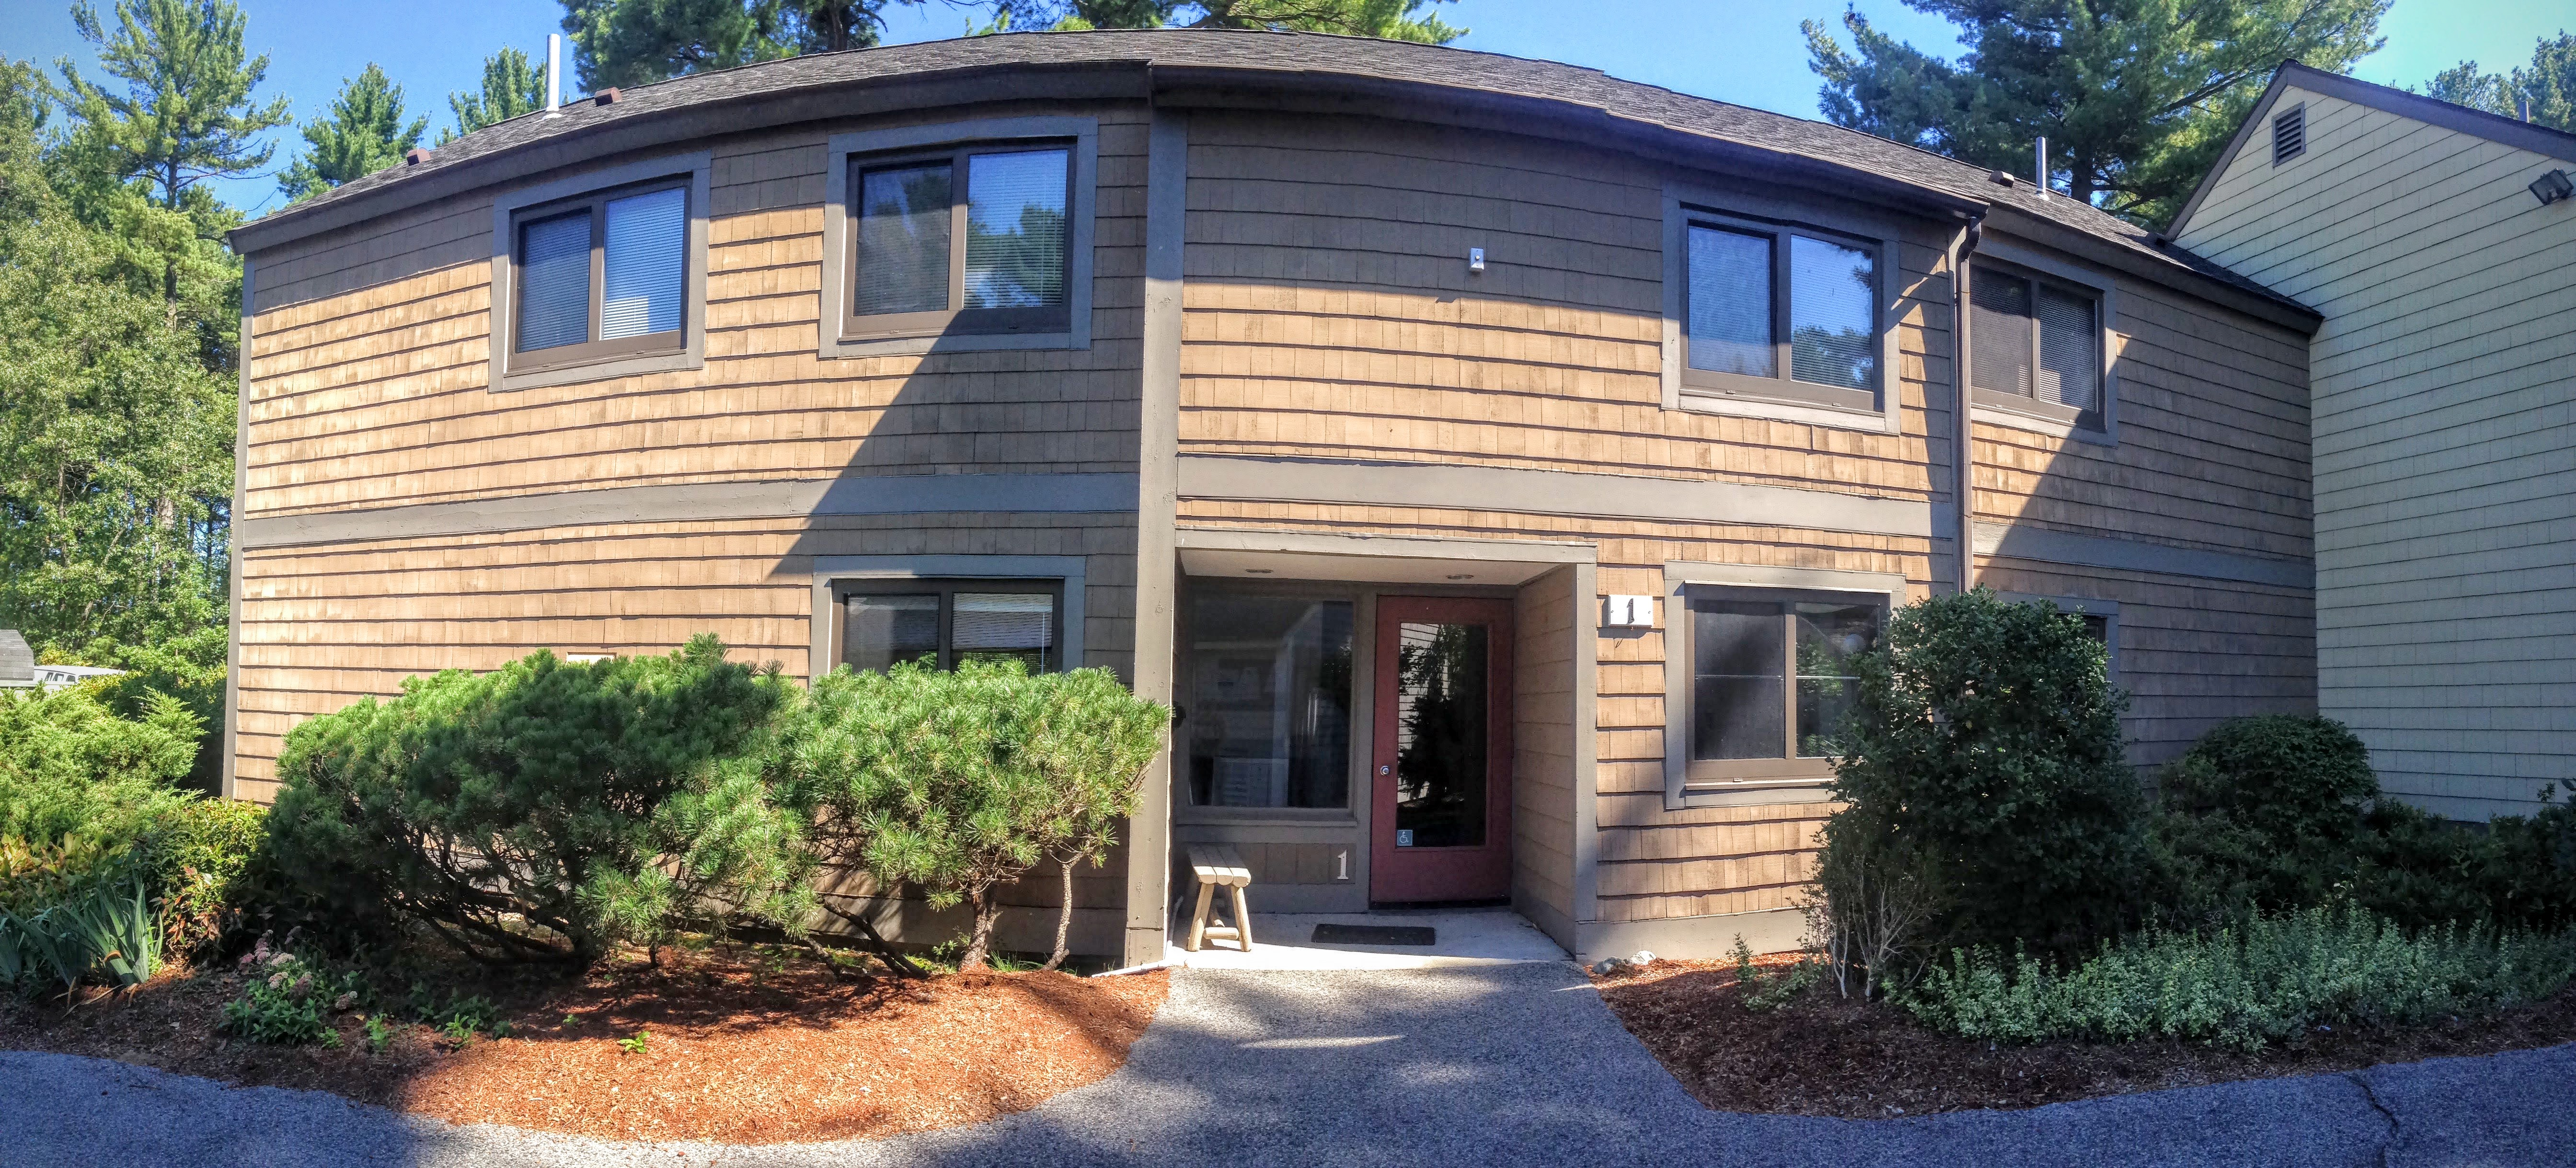
\includegraphics[width=0.75\textwidth]{findingschapter/sudburypanorama}
\caption{Duplex at the Sudbury Public Housing Development}
\end{figure}

\subsubsection{The Introduction of Renewable Technology to the Sudbury Public Housing Development}
\par In order to reduce this electricity cost the DHCD applied for funding through the DOER to fund a pilot program for the Sudbury Public Housing Development to replace the electric baseboards in four apartments with Air Source Heat Pumps (ASHPs). Since the DHCD is concerned with saving money for the state, they did not have a feasibility study commissioned for this renovation. Four ASHPs were installed within the Sudbury Public Housing Development with a grant from the DOER providing 100\% of the \$32,550 project cost.
\begin{figure}[H]
\centering
\includegraphics[width=0.75\textwidth]{findingschapter/sudburyoutsideunits}
\caption{ASHP’s at Sudbury Public Housing Development}
\end{figure}

\subsubsection{Timeline}
\par A typical installation of four ASHPs should take about a week to complete. Due to the need to secure funding, the state requirement is to source the lowest bid for the installation. With a conflict with one resident not wanting the system installed in their unit and an atypical installation process, the Sudbury Public Housing Development took 1.5 years from start to finish.
\begin{figure}[H]
\centering
\includegraphics[width=0.75\textwidth]{findingschapter/sudburyinsideunit}
\caption{Indoor ASHP vent at Sudbury Public Housing Development}
\end{figure}

\subsubsection{Resident Feedback}
\par Aside from one resident who wished to not have the system installed in their unit, the feedback from the residents has been positive. One resident spoke very highly of the new system and the reliable heating, cooling, and dehumidification it provides. He is quoted as saying that “it is the best invention ever” and that he “wished it had been around 50 years ago.” When asked about the maintenance of the system, he explained that all he does to maintain the systems is clear out the filters every three months, though the manufacturer recommended maintenance is to clean the filters every six months. This resident also mentioned that he has helped others to clean their filters as well. A second resident voiced that while she has heard good things about the systems, she knows that some residents struggle with the remote control that is used to change settings. She mentioned that there are different types of remotes in the different units, and that some people wish they were taught how to use it. Once the four pilot units had been installed and online, the focus of the project shifted toward metering the performance of the ASHPs.

\subsubsection{PowerWise Metering}
\par The Sudbury Public Housing Development installed a metering tool, PowerWise, to measure the electricity usage of units with ASHPs and compare to the electricity usage of the control units. Other public housing developments have installed ASHPs, but have not been able to effectively monitor the energy savings due to a lack of accurate and specific data. In the previous installations, the only accessible information was the billing information from an entire building’s electricity use. From this, the DHCD has been able to estimate how much money the installation of the ASHPs has been saving them, but they do not have concrete data on what percentage of the savings are actually coming from the switch to ASHPs. Sudbury was to be the test site for their new metering technology to obtain that missing data.
\par The PowerWise metering system was first installed in four cold climate one-to-one air source heat pumps, and four control units with electric baseboard heat. This was done to determine the baseline KWH usage over a full year by comparing the four pilot units with the four control units. However, due to the manner of ASHP installation and difficulties with unorganized circuit breakers, the DHCD hadn’t been able to obtain and analyze the data.  In September, 2015, the PowerWise engineers worked with the DHCD engineer in an effort to correct the wiring mistakes in order to produce accurate and usable data for the pilot and control units. However, due to the nature of the older buildings and the complicated circuitry, this took several attempts. As of 9/17/2015, the electricity usage is said to be accurate. Due to the late availability of accurate data, we were not able to provide substantial data analysis regarding electricity usage trends and cost savings.

\subsubsection{Lessons Learned}
\par From our interview and onsite visit at the Sudbury Public Housing Development, we developed a list of “lessons learned” that is included in our case studies. The first lesson learned is the importance of commissioning a feasibility study. There was no feasibility study commissioned at the Sudbury Public Housing Development, and feasibility studies provide not only recommendations for the specifics of the renewable technology to be installed, but in many cases also provide background information on the building/units themselves. Had this study been conducted, the many challenges of installing a pilot program and working with PowerWise in this situation would have been exposed.

\subsubsection{Site Summary}
\par There are a number of qualities about the Sudbury housing development that make it unsuitable for a pilot program to determine the effectiveness of a new technology. First, the tenants at Sudbury have fairly irregular usage habits. This site becomes more unsuitable when we add the fact of Sudbury not having any historic, per-unit power usage data. Another issue is that the tenants were not instructed on how to use new technologies, and since they control the temperature in their own apartment, this caused more irregularities in the metering and effectiveness of the systems. There also isn’t a maintenance plan for the new systems, which places the responsibility of maintaining the ASHPs on the tenants.
\par Several issues can be worked around by effectively educating the tenants about the systems being installed in their homes and setting up the appropriate infrastructure. The tenants that had the new systems installed in their apartment at Sudbury were not instructed on how to use or maintain their new ASHPs. In fact, not even the housing director was given any instruction on the operation or maintenance of the systems. The control for an ASHP is more complex than a traditional thermostat, but if it is explained to the tenants, it can be just as easy to use. In a more complete installation where every unit in the housing development is upgraded, the responsibility of maintenance would become a routine for the facilities staff and no longer fall to the tenants. In the realm of electricity usage metering, a full installation would increase the sample size and possibly normalize out some the outliers from the data. The issues with the tenants and the lack of historical data just point to the answer that Sudbury should not have been chosen as the primary metering site.

\section{Site Findings}
\par After we interviewed stakeholders and project leaders from each project site we studied, we noticed that each project process was complex in its own way, and each project involved different successes and challenges. We compiled the following findings after analyzing the interview transcripts and feasibility studies from each project site. Included with each finding is information and evidence from various project sites.
Site Findings:
  \begin{itemize}
    \item{Commissioning a Feasibility Study Prior to Beginning a Renewable Thermal Project Can Be Very Valuable}
    \item{Failure to Consider the Context in which a Renewable Energy Technology is being Implemented can Lead to Poor Performance and Increased Required Maintenance}
    \item{Educating the Community about New Technology before Installation can Lead to Community Support}
    \item{Working with Experienced Engineers Can Make a Big Difference In The Project Timeline and Post Project Effectiveness}
    \item{Improving a Building’s Energy Efficiency Improvements Prior to or in Addition to Upgrading the Heating System Leads to Increased Cost Savings}
    \item{Public Housing Rules and Regulations Can Be Barriers When Implementing a Renewable Technology Project}
    \item{Failure to Consider Context when Choosing a Metering System can Lead to Problems with Gathering Data}
  \end{itemize}

\subsection{Commissioning a Feasibility Study Prior to Beginning a Renewable Thermal Project Can Be Very Valuable}
\par For many renewable thermal project sites working with DOER funding, the first step in the process is to commission a feasibility study from an engineering firm. These feasibility studies provide information pertaining to the specific project site including cost estimates of project construction, estimated payback period or break even point, renewable technology sizing recommendations, and annual comparisons of fossil fuel cost to renewable energy technology fuel cost.
\par These feasibility studies can prove to be very valuable resources when beginning a renewable thermal project. Along with providing information regarding various aspects of the project, the investigative work needed to produce these studies can also uncover underlying issues within the building that were not previously known such as the presence of asbestos, poor insulation, and energy management system efficiency problems. In the following sections, we provide evidence for this finding from each project site

\subsubsection{Amherst College Bunker Building}
\par When Amherst College learned of the grant opportunities from the DOER and that their oil boilers were reaching the end of their life expectancy, they commissioned a feasibility study to be completed comparing the initial cost and fuel cost of installing a propane boiler system and a biomass boiler system. This feasibility study aided in making their decision to work with the biomass boiler system as it showed that using a biomass boiler system would be more cost effective and could sufficiently provide heat to meet their usage needs.(Kohler, 2014; Amherst College, 2014)

\subsubsection{Southern Berkshire Regional School}
\par Southern Berkshire Regional School District (SBRSD) commissioned a feasibility study from BEAM engineering before contacting potential contractors in order to determine if biomass boilers would be functional in the school. This feasibility study provided a cost estimate of the project, general boiler technology information, general construction process information, a comparison of fossil fuel costs and biomass pellet costs as well as two different options regarding boiler sizing and oil boiler backup logistics. Not only did this feasibility study provide the SBRSD with a general understanding of what this project would involve, but the SBRSD was also able to use this feasibility study as informational material when looking for contractors to complete the construction.  While the selected contractors, RDK Engineering, conducted their own research to produce a second feasibility study, this first feasibility study provided RDK with basic information regarding the project so that they could determine if they were well suited for the project as a contracting firm.
\par Once RDK produced their own feasibility study, the SBRSD and the DOER noticed a few discrepancies between the two feasibility studies. The BEAM feasibility study and the RDK feasibility study did not agree on some aspects of the project including boiler sizing and boiler room configuration. Since the SBRSD had commissioned these two feasibility studies with the help of the DOER, they had the opportunity to be proactive and commission a third feasibility study which produced more consistent information regarding project specifics. (BEAM Engineering, 2014; D.C. Architects, 2014;RDK Engineers, 2014, Wilson Engineering, 2015)

\subsubsection{Sudbury Public Housing Development}
\par The Sudbury Public Housing Development did not commission a feasibility study when implementing the pilot Air Source Heat Pump project. There were many unknowns throughout the project process and the installation of some units needed to be adjusted after the initial installation. It was also unknown at the beginning of the project whether or not the use of ASHPs in this setting would be cost effective compared to the existing electric baseboard heating system. If a feasibility study had been commissioned, more information would have been known been known about this application of ASHPs and these issues may have been avoided.

\subsection{Failure to Consider the Context in which a Renewable Energy Technology is being Implemented can Lead to Poor Performance and Increased Required Maintenance}
\par Similarly to how various types of renewable technology are different, no two buildings are exactly alike. Moreover, each building is used for a different purpose and houses different types of people doing different activities. After investigating different aspects of the project processes at each different project site, analysis revealed that not considering the context of the renewable technology before beginning construction can lead to poor project performance and increased required maintenance. Furthermore, we learned that when the context of the renewable technology is considered prior to project implementation, the project runs more smoothly. Evidence of this finding from each project site is presented in the following sections.

\subsubsection{Amherst College Bunker Building}
\par The Amherst College bunker building is certainly a unique building with unique heating requirements. Unlike a usual school building, the bunker building is climate controlled year round to maintain the physical integrity of the books it houses. Also, the bunker building is below grade. This means that the heating load would remain relatively constant between the winter and summer months since the earth surrounding the bunker building maintains a mostly constant temperature. Fortunately, these factors were considered when purchasing appropriately sized boilers and accompanying silo.
\par Aesthetics was considered when planning the biomass boiler system installation at the bunker building. A new above grade boiler building was constructed to house the boilers adjacent to the new silo. Since the bunker building is off campus, the issue of silo aesthetics was not a problem. However, the individual we interviewed stated “I don’t think we would get away with putting a silo in the campus,” highlighting the importance of considering the application of the technology when planning the design.
\par Another aspect of the biomass boiler system installation that was considered at Amherst College was who would be maintaining the new boilers and how they would be maintaining them. With such a large campus, Amherst College has a robust maintenance plan with sufficient staff members. Before the system was installed, the maintenance team became familiar with the maintenance requirements of biomass boilers in order to determine if their staff would be capable. The boilers they chose provide updates regarding any maintenance needs via the internet which decreases the learning curve of maintaining a new system. The maintenance team is also planning on working with Froling Engineers during the first annual maintenance. The plan is that the Amherst College maintenance staff will use this opportunity to learn how to complete the annual maintenance, and after the first year, will begin to do the annual maintenance on their own. This maintenance requires turning the boiler off, however, Amherst College has two boilers with 100\% redundancy each, this means there will be no gap in climate controlling in the building while the maintenance process takes place.

\subsubsection{Southern Berkshire Regional School}
\par When determining which renewable thermal technology would be best applicable in the context of the Southern Berkshire Regional School, many factors were considered. Very quickly, geothermal heat pumps were eliminated as an option due to the large upfront cost. When looking into biomass boilers as an option, the school made sure to look into how this system would affect air quality and whether or not the boilers would produce unpleasant noise. In a school setting, air quality is very important, as children spend a big portion of their days there. Noise is also a concern for schools because they don’t want anything distracting students from their education. Fortunately, biomass boilers are comparable in terms of noise to oil boilers, which the school previously used to heat the building, and do not affect air quality in the classrooms as they burn very cleanly.
\par In our sponsor at the DOER’s experience, many schools have concerns regarding the aesthetics of the biomass pellet storage silo. Fortunately, this was considered when designing the layout of the new system, and it was deemed possible to place the biomass silo in the back of the building near the boiler room, where it would not be visible from the street.
\par One aspect of the project that was not considered as heavily when planning the project was maintenance. Unlike Amherst College, the Southern Berkshire Regional School is a public school with only one building and thus a need for smaller maintenance staff. Whereas the maintenance staff at Amherst College is more experienced with robust boiler systems in different buildings across campus, the maintenance staff at Southern Berkshire Regional School is not as technically savvy, as this has not been a requirement to satisfy the school’s maintenance needs. The SBRSD also did not make a maintenance plan or contract for once the boilers are on line. They are currently concerned with who will maintain the new boilers and how they will learn the proper maintenance techniques. One individual we interviewed from the SBRSD states in regards to the biomass boiler system “who will maintain it? Who has the expertise in these types of boilers to maintain it, and then it’s going to be a little bit of a learning curve for our maintenance staff to learn how to operate and all that, so that was one of the concerns.” This concern also highlights the importance of considering all aspects of the renewable technology application for each site, including the people who will be working with the technology.

\subsubsection{Sudbury Public Housing Development}
\par Since the Sudbury Public Housing Development was concerned with quickly reducing their electricity costs per unit, there were a lot of aspects about this particular context of ASHPs that were not considered or planned for.
\par The first aspect of applying ASHPs in a public housing development that was not considered was how a community of mostly elders would respond to and use the ASHPs. Many of the elderly residents were not familiar with ASHPs and thus some residents responded negatively to the idea of having this new technology placed in their units. After the ASHPs were installed and the PowerWise metering system was being implemented, many of the residents became upset with the electricians coming in and out of their units and moving their belongings. Since the residents were not educated on how to use the ASHPs, they used them like they would an electric baseboard heating system with a thermostat: by turning it on and off to maintain their comfort level. However, ASHPs function best and is the most energy efficient when set to a temperature and left on automatic mode. Using an ASHP like an electric baseboard heating system increases the operating cost and decreases the effectiveness of the system. The individual we interviewed that worked closely with the PowerWise system states “that is one of the concerns we have in elderly units. This is not a thermostat that you dial forward and backwards. It’s a handheld remote control and it has the options to keep the system in heating, cooling, and even dehumidification. So you have to choose the right mode.”
\par Another aspect of the public housing development application of ASHPs that was not considered and poses as an issue is maintenance. Since only four units at the housing development have had ASHPs installed, the maintenance of these systems hasn’t been integrated into the housing developments maintenance plan. The filters in the unit need to be cleaned out every six months, and this responsibility is left to the residents. One resident doesn’t mind the maintenance and he helps out the other residents who either don’t know how to or are unable to maintain their systems themselves.

\subsection{Educating the Community about New Technology before Installation can Lead to Community Support}
\par Since most of the DOER’s grant money goes to public organizations, ensuring that the projects have the support of the community is very important. In most cases, the DOER’s contribution only partially funds these projects, so it is up to the community members who use these public buildings to pay for any work on them in the form of local taxes. Lack of community support can be a barrier to both implementation and effective operation. We found that educating the community about the new technology before installation can lead to community support. In the following sections, we present evidence of this finding from each project site where it was applicable.

\subsubsection{Southern Berkshire Regional School}
\par The Southern Berkshire Regional School District received grants totalling around 40\% of the total project cost. This meant that the remainder of the project was to be funded using the taxpayer’s contributions. Even though the money would be going to improve the local school building, the community members were hesitant to approve the spending. This almost prevented the project from being implemented.
\par By providing effective education and instruction to the community, the Southern Berkshire Regional School District was able to obtain the community support necessary for the project to move forward. According to one of the two individuals we interviewed who worked very closely with acquiring the grants from the DOER, the school district “brought a [biomass] expert to have him participate in several meetings so that the public could be educated.” In addition, there was a community press release that showed breakdown of taxpayer increases per year because of the renovation. For this community, this method worked to ease the minds of the taxpayers that this project could be paid for with only a minor increase in taxes each year. Through information on the technology and on the personal impact, the Southern Berkshire Regional School District was able to secure support and funding for their renovation.

\subsubsection{Sudbury Public Housing Development}
\par At the Sudbury Public Housing Development, the installation of the ASHPs was fully funded by the DOER, and the DHCD went ahead with the installations without first gaining support from the tenants. This has proven to be an issue with regards to operation and maintenance of the ASHPs. Since the tenants were never instructed how to operate or maintain their units, there have been complaints about the technology including one tenant who demanded that ASHP be removed from his unit. Some tenants also expressed that they did not believe that the new systems would work, and once it was installed, they confused the unpleasant sound of the previously installed water heater with the ASHPs.
\par The Sudbury Public Housing Development, while not proactive about educating their tenants, did eventually provide maintenance instructional materials to the tenant who asked for them. That tenant eventually went and personally taught the other tenants how to operate their ASHPs. Prior to the education, they were incorrectly controlling the units, which caused much more energy to be used. Instead of leaving the ASHPs in automatic mode, some tenants were turning the ASHPs on and off which causes a greater power consumption.
\par It is important for people to know that the new system they are implementing actually works. When the community trusts and understands the system, there will in some cases be more support for it and in some cases more efficient operations and maintenance. The management of all of the projects we investigated found it useful to visit other sites that have installed similar technologies. Seeing proof of it working for another community boosts the trust in the technology. The housing director at Sudbury told us that “just hearing from other tenants about it and the comfort level that you /[a tenant/] felt… is the best recommendation.” Even hearing the stories of other sites, in a case study for example, can serve this purpose for many sites in the planning phases.

\subsection{Working with Experienced Engineers Can Make a Big Difference In The Project Timeline and Post Project Effectiveness}
\par Since the implementation of renewable thermal technologies for heating and cooling systems is just starting in Massachusetts, there are not many engineers that are familiar with these systems. Working with experienced engineers on this type of project makes a big difference to the success of the project. In the following sections, we provide evidence from each of the three case studies that support this finding.

\subsubsection{Amherst College Bunker Building}
\par Amherst College was recommended, by the DOER, to contract Froling, an Austrian company that has more than four decades of experience in wood heating technology. Since Amherst worked with a firm that is considered the “pioneers” in this field, their construction phase went almost perfect. They did not have many discrepancies when deciding what type of system to install, Since Amherst College worked with experienced engineers, they were well prepared for any unknown obstacle. During the construction phase, they suffered from a harsh winter that produced a delay in the timeline of the project. Nevertheless, this delay was minimal and they were not really affected in terms of cost or comfort.
\par Another benefit of working with experience engineers is that once the system is running they would try to assist you in any situation. Froling Company has been contracted to do the first annual maintenance, and helping Amherst College maintenance staff take care of the system. Furthermore, Froling Company keeps monitoring the system through the internet, informing Amherst College know if there is any problem with the boilers. Working with experienced engineers is a very important factor since it makes big difference during and after the project implementation. The individual we interviewed from Amherst College said that working with Froling Company has been the best decision since wood heating for this company “is their bread and butter”.

\subsubsection{Southern Berkshire Regional School}
\par Southern Berkshire Regional School District is an example of how important the engineer's experience is. As mentioned before SBRSD selected RDK Engineering as their contractors. This company did not have much experience with renewable thermal technology, and decided to conduct their own feasibility study. SBRSD and RDK feasibility study had a few differences that cause the project planning phase to get delayed. Due to these differences SBRSD and the DOER were able to bring a third party, Wilson Engineering which had more engineer experience than RDK, to produce a third and more accurate feasibility study.
\par After settling the discrepancies among the feasibility studies, SBRSD was able to continue their project and start the construction phase. The bid was given to RDK Engineers and due to the delays of solving the differences among the studies, the oil boilers were not ordered on time, and so the project timeline is behind schedule. This is an example of how important the contractors engineering experience is, and how contracting firms that does not know about this type of technologies could make a project timeline set behind.

\subsubsection{Sudbury Public Housing Development}
\par Since Sudbury Public Housing  Development is owned by the government they needed to accept the contractor who offered the lowest bid. Sometimes contractors who offer lower price quotes will not have as much engineering experience as those who offer a higher price quote. In this case they had several setbacks during their implementation process. One of these setbacks was that the contractors were not HVAC engineers; they were electricians and they are not familiar with this type of system. Thus, the system was not installed correctly the first time and electricians had to keep going into the tenant's room to fix it.

\subsection{Improving a Building’s Energy Efficiency Improvements Prior to or in Addition to Upgrading the Heating System Leads to Increased Cost Savings}
\par Making improvements to a building’s energy efficiency can significantly affect the amount of energy that the building is spending and combining this with a renewable source of energy for cooling and heating can not only result in less energy spent in this sector but also in reduced costs. The Southern Berkshire Regional School had a energy management system renovation in 2010, this made the building more energy efficient. In addition, this project was funded by DOER grants.“Annually we’re looking at savings of 3,508 gallons of heating oil because of these changes...” said one individual we interviewed who worked closely with increasing the building’s energy efficiency (Southern Berkshire Regional School District, 2010).

\subsection{Public Housing Rules and Regulations Can Be Barriers When Implementing a Renewable Technology Project}
\par While investigating different aspects of the project process at the Sudbury Public Housing Development, we learned that public housing rules and regulations, while they serve their purpose, can be barriers when implementing a renewable technology project. A requirement of public housing developments is that when they are undergoing a construction project that is estimated to cost more than \$10,000, they must put the project up to public bid, and accept the lowest bid they receive. While this method is effective at ensuring the public housing development saves money on a project, it also means that the electrician with the lowest bidder was not necessarily the most competent or familiar with ASHPs and their installation. This lack of experience with relatively new ASHP technology lead to several setbacks in the timeline of the installation as well as several instances of correcting mistakes, which involved entering the residents’ units, a slightly invasive process.

\subsection{Failure to Consider Context when Choosing a Metering System can Lead to Problems with Gathering Data}
\par Metering systems can be extremely useful for getting detailed information on energy usage of a house or other building. There are however many things to consider when looking into using a metering system for a certain application. One consideration is that the site must have reliable internet access if the system is to upload its data to a remote server. The Sudbury Public Housing Development did not correctly evaluate the effectiveness of a metering system at their complex.
\par The public housing complex in Sudbury is not well suited for an internet based metering system for many reasons. There is inconsistent connection to the internet because the housing development is in a somewhat rural location. Additionally, public housing developments in general aren’t practical applications for a small scale pilot program using a metering system due to the wide range of tenant behaviors that will skew the data. A requirement of the PowerWise metering system is that the breaker panel be organized to accurately connect and label individual circuits. However, the breaker panels at Sudbury were very disorganized, having had many changes in the 50 years they’ve been in service. Had the Sudbury Public Housing Development properly evaluated the application they were looking at implementing this metering system in, they may have realized the pitfalls before installing it.